% =============================================================================
% Evaluación de paradigmas de scheduling en sistemas OFDMA
% bajo tráfico y condiciones espaciales heterogéneas
%
% Formato: IEEE Conference Proceedings (IEEEtran)
% Compilar: pdflatex main.tex && bibtex main && pdflatex main.tex (×2)
%           o usar: make
% =============================================================================

\documentclass[conference]{IEEEtran}

% Paquetes
\usepackage[utf8]{inputenc}
\usepackage[T1]{fontenc}
\usepackage[spanish]{babel}
\usepackage{amsmath,amssymb}
\usepackage{graphicx}
\usepackage{booktabs}
\usepackage{multirow}
\usepackage{array}
\usepackage{url}
\usepackage{cite}
\usepackage{xcolor}
\usepackage{float}
\usepackage{caption}
\usepackage{subcaption}
\usepackage{siunitx}
\usepackage{microtype}

\graphicspath{{figures/}}

% Metadatos
\title{Evaluación de Paradigmas de Scheduling en Sistemas OFDMA bajo Heterogeneidad Espacial y de Tráfico}

\author{
  \IEEEauthorblockN{Alfonso García}
  \IEEEauthorblockA{
    Maestría en Ciencias de la Computación\\
    Benemérita Universidad Autónoma de Puebla\\
    Puebla, México\\
    \texttt{alfonso.089911@gmail.com}
  }
}

\begin{document}

\maketitle

% =============================================================================
\begin{abstract}
El scheduler de enlace descendente es, en la práctica, el componente que decide si
un usuario en el fondo de la celda recibe datos o queda ignorado mientras el vecino
del frente monopoliza el canal. Elegir cuál paradigma usar no es trivial: siete
algoritmos bien conocidos ---clasificados según la taxonomía de Capozzi
et al.~\cite{capozzi2012}--- se comportan de manera radicalmente distinta en función
de cómo están distribuidos los usuarios y qué tipo de tráfico generan.

Este trabajo ejecuta 1{,}680 simulaciones en ns-3.47/LTE para cuantificar esas
diferencias bajo cuatro condiciones combinadas de heterogeneidad espacial y de tráfico.
Dos hallazgos van contra la intuición inicial: primero, la distribución clusterizada
de usuarios afecta menos la equidad de lo esperado ---la carga de la celda es el
factor dominante para 6 de 7 schedulers---; segundo, M-LWDF, el algoritmo que
más agresivamente protege los flujos con garantía de servicio (GBR), es también el
que más reduce el throughput total de celda cuando el tráfico es heterogéneo ($-31\%$).
Lo que sí confirman los datos con alta significancia ($p<0.001$, $d\approx5$) es que
M-LWDF y PSS superan a PF en equidad global cuando los usuarios están clusterizados
y el tráfico mezcla GBR con best-effort: un resultado que tiene implicaciones directas
para el despliegue en escenarios de tipo URLLC en redes LTE/5G.
\end{abstract}

\begin{IEEEkeywords}
OFDMA, scheduling, LTE, fairness, QoS, heterogeneidad espacial, tráfico heterogéneo, ns-3
\end{IEEEkeywords}

% =============================================================================
\section{Introducción}

Imagine una sala de espera hospitalaria conectada por LTE: algunas personas transmiten
video de consulta telemédica (requieren baja latencia y bitrate garantizado), otras
descargan datos de historiales (best-effort), y todos están físicamente agrupados lejos
de la antena. El scheduler de la estación base debe decidir, cada milisegundo, a quién
darle recursos. Esa decisión no es trivial, y su impacto sobre la experiencia de cada
usuario depende tanto del algoritmo elegido como de las condiciones del entorno.

El problema de asignación de recursos en OFDMA ha generado docenas de propuestas
desde los primeros años de LTE. Los tres clásicos ---Round Robin, Maximum Throughput
y Proportional Fair--- están documentados con precisión \cite{pf1999}. Capozzi et
al.~\cite{capozzi2012} organizaron la literatura en una taxonomía de cinco categorías
que es hoy el marco de referencia estándar. El problema es que casi toda esa literatura
evalúa los schedulers en condiciones ideales: usuarios distribuidos uniformemente en la
celda, tráfico homogéneo, un único tipo de servicio. En la práctica, los usuarios se
agrupan geográficamente (hay más personas en el centro comercial que en el
estacionamiento), y en la misma celda coexisten video, voz, gaming y tráfico de fondo.

Lo que no existe, hasta donde encontramos, es una evaluación sistemática que aísle
por separado el efecto de la distribución espacial y el de la mezcla de tráfico sobre
la \emph{taxonomía completa} de schedulers, con suficientes repeticiones estadísticas
para afirmar diferencias con confianza. Ese es exactamente el experimento que reportamos
aquí: 7 schedulers, 4 condiciones combinadas, 20 repeticiones por configuración, en
total 1{,}680 simulaciones en ns-3.47.

Los resultados tienen algunas sorpresas. Anticipábamos que los clusters de usuarios
harían colapsar la equidad de los schedulers orientados a throughput, pero la realidad
resultó más matizada. La distribución espacial importa menos de lo esperado; la carga
de la celda importa más. Y M-LWDF, el más sofisticado de los algoritmos QoS-aware,
resulta ser también el que más castiga el throughput total cuando el tráfico es
heterogéneo. Discutimos por qué tiene sentido, y qué significa para la elección de
scheduler en escenarios reales.

% =============================================================================
\section{Marco Teórico}
\label{sec:marco}

\subsection{OFDMA y asignación de recursos en LTE}

En LTE, el espectro de 10~MHz se divide en 50 bloques de recursos (RBs) de 180~kHz.
En cada TTI, el scheduler asigna RBs a usuarios según el canal reportado mediante
el indicador de calidad de canal (CQI). El CQI refleja la relación señal-a-interferencia-
más-ruido (SINR) en cada RB, permitiendo a los schedulers channel-aware explotar la
diversidad multiusuario \cite{lte3gpp}.

\subsection{Métricas de evaluación}

\textbf{Throughput de celda} ($T_c$): suma del throughput por usuario en Mbps.

\textbf{Índice de Jain} ($J$): medida de equidad de asignación de recursos \cite{jain1984}:
\begin{equation}
  J(x_1,\ldots,x_n) = \frac{\left(\sum_{i=1}^{n} x_i\right)^2}{n \cdot \sum_{i=1}^{n} x_i^2}
  \label{eq:jain}
\end{equation}
donde $x_i$ es el throughput del usuario $i$. $J \in [1/n, 1]$; $J=1$ indica equidad perfecta.

\textbf{Retardo E2E} ($D$): retardo medio extremo a extremo por flujo IP (FlowMonitor).

\textbf{PLR}: tasa de pérdida de paquetes = $(N_{tx}-N_{rx})/N_{tx}$ por flujo.

\subsection{Taxonomía de Capozzi}

Capozzi et al.~\cite{capozzi2012} clasifican los schedulers LTE en cinco categorías.
Este trabajo activa las tres relevantes para redes heterogéneas:

\begin{itemize}
  \item \textbf{(i) Channel-unaware / QoS-unaware}: no utiliza CQI ni restricciones de
        QoS. Representantes: RR, BET.
  \item \textbf{(ii) Channel-aware / QoS-unaware}: explota CQI pero no distingue
        tipos de flujo. Representantes: MT, TTA, PF.
  \item \textbf{(iii) Channel-aware / QoS-aware}: combina CQI con restricciones de
        delay/bitrate por flujo. Representantes: M-LWDF, PSS.
\end{itemize}

Las categorías (iv) semi-persistent y (v) energy-aware se descartan por tener
objetivos de optimización incompatibles con las métricas evaluadas.

\subsection{Algoritmos evaluados}

La Tabla~\ref{tab:schedulers} resume los siete schedulers. Las métricas clave son:

\textbf{PF}: $m_i(t) = r_i(t) / \bar{r}_i(t)$ donde $r_i(t)$ es la tasa instantánea y
$\bar{r}_i(t)$ el throughput histórico promedio.

\textbf{M-LWDF}: $m_i(t) = -\log(\delta_i) \cdot D_i(t) \cdot r_i(t) / \bar{r}_i(t)$
donde $\delta_i$ es la PLR objetivo y $D_i(t)$ el delay HOL \cite{mlwdf2001}.

\textbf{PSS}: asignación en dos etapas --- TDPS prioriza UEs GBR con delay elevado;
FDPS aplica PF dentro del grupo seleccionado \cite{pss2006}.

\begin{table}[t]
  \centering
  \caption{Schedulers evaluados --- esquema 2-3-2 de la taxonomía Capozzi}
  \label{tab:schedulers}
  \footnotesize
  \begin{tabular}{@{}llll@{}}
    \toprule
    \textbf{Scheduler} & \textbf{Cat.} & \textbf{Clase ns-3} & \textbf{Característica} \\
    \midrule
    RR     & (i)   & RrFfMacScheduler     & Tiempo igual por UE \\
    BET    & (i)   & FdBetFfMacScheduler  & Throughput igual por UE \\
    MT     & (ii)  & TdMtFfMacScheduler   & Maximiza tasa instantánea \\
    TTA    & (ii)  & TtaFfMacScheduler    & Normaliza por tasa wideband \\
    PF     & (ii)  & PfFfMacScheduler     & Proporcional histórico \\
    M-LWDF & (iii) & MlwdfFfMacScheduler  & Delay HOL + canal (impl.) \\
    PSS    & (iii) & PssFfMacScheduler    & Separación GBR/non-GBR \\
    \bottomrule
  \end{tabular}
\end{table}

% =============================================================================
\section{Estado del Arte}
\label{sec:arte}

La referencia más influyente sigue siendo Capozzi et al.~\cite{capozzi2012}, que
evaluaron doce schedulers con distribución uniforme de usuarios y tráfico full-buffer.
Sus resultados para PF con N=20 reportan Jain$\approx$0.82, un valor notablemente
superior al 0.747 que observamos aquí con fading EPA activo. La diferencia no es
menor: sin fading, los UEs equidistantes tienen CQI idéntico y PF se comporta casi
como RR. Con fading real, PF explota la diversidad temporal y favorece a quien tiene
mejor canal \emph{en ese instante}, lo que degrada la equidad global.

Andrews et al.~\cite{mlwdf2001} propusieron M-LWDF originalmente para redes 1xEV-DO,
con foco en mantener la tasa de pérdida de paquetes por debajo de un umbral estadístico.
Su extensión a LTE demostró ventajas en latencia para flujos de video, aunque los
experimentos originales usaban modelos de tráfico ON-OFF con tasas moderadas ---muy
distintas al escenario de saturación total que evaluamos aquí.

PSS \cite{pss2006} introduce la idea de separar el scheduler en dos etapas (TDPS para
GBR, FDPS para el resto), que en teoría permite servir a ambas clases sin competencia
directa. En la práctica, los resultados de Sesia et al. muestran ventajas principalmente
bajo carga media; bajo saturación plena, la separación no es tan clara porque los
recursos del FDPS se agotan rápidamente.

Trabajos más recientes comparan schedulers bajo heterogeneidad de tráfico
\cite{tta2007,bet2004}, pero normalmente con N fijo y distribución uniforme, o con
distribución clusterizada pero tráfico homogéneo. No encontramos ninguno que cruce
ambas dimensiones ---distribución espacial y mezcla de tráfico--- sobre la taxonomía
completa, con 20 repeticiones estadísticas por configuración para controlar la
varianza del fading.

% =============================================================================
\section{Metodología}
\label{sec:metodo}

\subsection{Entorno de simulación}

Usamos ns-3.47 con módulo LTE/EPC (Tabla~\ref{tab:params}). Tres decisiones de
configuración merecen justificación explícita.

\textbf{Fading EPA en lugar de canal puramente determinístico.} Sin fading, dos UEs
a la misma distancia del eNB tienen CQI idéntico en cada TTI. PF se convierte casi
en RR y las diferencias entre schedulers channel-aware se minimizan artificialmente.
El modelo TraceFadingLossModel con traza EPA 3~km/h añade variación temporal por RB,
lo que permite a MT y PF explotar diversidad multiusuario real. Sin esto, el experimento
no tendría sentido.

\textbf{Tráfico full-buffer en T1.} Una versión temprana del experimento usó CBR a
1~Mbps por usuario. El resultado fue que en varios TTIs la cola de algunos UEs estaba
vacía ---el scheduler no tenía qué asignar--- y las diferencias entre algoritmos
desaparecían en el ruido. Cambiar a OnOff always-on a 10~Mbps/UE garantiza que la
demanda supera siempre la capacidad de la celda ($\approx$20~Mbps), forzando al
scheduler a elegir activamente en cada TTI.

\textbf{Asignación interleaved en T2.} Si los UEs de video se concentran en un cluster
y los BE en otro, es imposible separar si un scheduler favorece video porque es QoS-aware
o simplemente porque esos UEs están más cerca de la antena. La asignación $u \bmod 3$
mezcla los tres tipos en cada cluster, haciendo la posición y el tipo de tráfico
estadísticamente independientes.

\begin{table}[t]
  \centering
  \caption{Parámetros fijos de simulación}
  \label{tab:params}
  \footnotesize
  \begin{tabular}{@{}ll@{}}
    \toprule
    \textbf{Parámetro} & \textbf{Valor} \\
    \midrule
    Simulador          & ns-3.47, módulo LTE \\
    eNodeBs            & 1 (celda única) \\
    Potencia TX eNB    & 46~dBm \\
    Frecuencia DL      & 2.1~GHz (EARFCN 100) \\
    Ancho de banda DL  & 10~MHz $\to$ 50~RBs \\
    Path loss          & Log-distance, $\alpha$=3.5 \\
    Fading             & TraceFadingLossModel EPA 3~km/h \\
    CQI                & Dinámico, full-bandwidth, 1~TTI \\
    EPC                & PointToPointEpcHelper \\
    Protocolo          & UDP extremo a extremo \\
    Duración           & 30~s (warmup 5~s descartado) \\
    Semilla RNG        & SetSeed(12345), SetRun(\emph{runId}) \\
    \bottomrule
  \end{tabular}
\end{table}

\subsection{Variables independientes y escenarios}

\textbf{Distribución espacial:}
\begin{itemize}
  \item \textbf{D1 --- Uniforme}: UEs distribuidos uniformemente en disco de radio 490~m.
  \item \textbf{D2 --- Clusterizada}: 3 clusters a distancias diferenciadas del eNB
        (C1=100~m, C2=250~m, C3=400~m), radio de cluster 70~m, ángulos separados 120°.
        Implementa la condición de canal heterogéneo explicitamente requerida.
\end{itemize}

\textbf{Tipo de tráfico:}
\begin{itemize}
  \item \textbf{T1 --- Homogéneo}: todos los UEs con tráfico full-buffer (OnOff a 10~Mbps).
        Capacidad ofrecida $\gg$ capacidad de celda ($\approx$20~Mbps), garantizando saturación.
  \item \textbf{T2 --- Heterogéneo}: asignación interleaved ($u \bmod 3$): video GBR (QCI-4,
        1.5~Mbps), gaming GBR (QCI-3, 64~kbps), best-effort full-buffer. La asignación
        interleaved garantiza que cada cluster recibe los tres tipos mezclados,
        eliminando correlación posición-tráfico.
\end{itemize}

\subsection{Diseño experimental}

El experimento completo comprende dos grupos:
\begin{itemize}
  \item \textbf{Grupo A} (H1, H2): 7 schedulers $\times$ D1/D2 $\times$ N$\in\{$10,20,40$\}$ $\times$ T1 $\times$ 20 runs = \textbf{840 corridas}.
  \item \textbf{Grupo B} (H3, H4): 7 schedulers $\times$ D1/D2 $\times$ N$\in\{$10,20,40$\}$ $\times$ T2 $\times$ 20 runs = \textbf{840 corridas}.
\end{itemize}

\textbf{Total: 1{,}680 corridas.} Cada configuración utiliza 20 repeticiones con semillas
independientes para obtener IC al 95\% (t-Student, $df=19$, $t_{crit}=2.093$).
Las comparaciones entre schedulers emplean el test de Welch con umbral $p<0.05$.

\subsection{Hipótesis de investigación}

\begin{itemize}
  \item[\textbf{H1}:] Los schedulers orientados a throughput presentan degradación no lineal de fairness bajo distribución clusterizada.
  \item[\textbf{H2}:] La heterogeneidad espacial tiene mayor impacto sobre fairness que el número de usuarios.
  \item[\textbf{H3}:] Los schedulers balanceados (PF) pierden eficiencia espectral cuando coexisten flujos GBR y best-effort.
  \item[\textbf{H4}:] Los schedulers híbridos (M-LWDF, PSS) mejoran el compromiso fairness-throughput frente a PF bajo tráfico heterogéneo.
\end{itemize}

% =============================================================================
\section{Resultados}
\label{sec:resultados}

\subsection{Escenario de referencia (N=20, D1, T1)}

Antes de analizar los efectos de la heterogeneidad, vale la pena observar el escenario
más simple: distribución uniforme, tráfico homogéneo, N=20. Los números de la
Tabla~\ref{tab:referencia} cuentan una historia ya conocida pero que el fading con
full-buffer hace más nítida.

MT alcanza 11.09~Mbps ---nada mal--- pero en la práctica solo está sirviendo a 6 de
20 usuarios. Los otros 14 reciben exactamente cero bytes durante los 25 segundos de
medición. Es la versión más cruda del trade-off throughput/fairness: el algoritmo
hace su trabajo perfectamente, maximiza la tasa instantánea, y en el proceso convierte
la celda en un monopolio. BET es el extremo opuesto: Jain=0.999 es casi perfectamente
justo, pero a costa de bajar el throughput de celda a 4.32~Mbps. PF, con 14.16~Mbps
y Jain=0.747, es el equilibrio que la mayoría de los operadores elegiría por defecto.

Lo que llama la atención de esta tabla es que PF y M-LWDF producen exactamente los
mismos números bajo T1. Tiene sentido: M-LWDF es PF más un término de delay HOL.
Con tráfico full-buffer todos los paquetes tienen delay similar, así que el término
extra no cambia nada. M-LWDF solo se diferencia cuando hay flujos con restricciones
de latencia distintas, es decir, bajo T2.

\begin{table}[t]
  \centering
  \caption{Métricas de referencia --- N=20, D1, T1 (media ± IC 95\%)}
  \label{tab:referencia}
  \footnotesize
  \begin{tabular}{@{}lcccc@{}}
    \toprule
    \textbf{Scheduler} & \textbf{Cat.} & \textbf{Tput [Mbps]} & \textbf{Jain} & \textbf{UEs activos} \\
    \midrule
    RR     & (i)   & 7.22 ± 0.60   & 0.642 ± 0.040 & 20/20 \\
    BET    & (i)   & 4.32 ± 0.27   & 0.999 ± 0.000 & 20/20 \\
    MT     & (ii)  & 11.09 ± 0.19  & 0.116 ± 0.023 & 6/20  \\
    TTA    & (ii)  & 10.04 ± 0.68  & 0.777 ± 0.035 & 20/20 \\
    PF     & (ii)  & 14.16 ± 0.84  & 0.747 ± 0.023 & 20/20 \\
    M-LWDF & (iii) & 14.16 ± 0.84  & 0.747 ± 0.023 & 20/20 \\
    PSS    & (iii) & 14.53 ± 0.91  & 0.707 ± 0.033 & 20/20 \\
    \bottomrule
  \end{tabular}
\end{table}

\subsection{H1: Fairness bajo distribución clusterizada}

La predicción de H1 era que los schedulers orientados a throughput degradarían su
fairness al pasar de distribución uniforme (D1) a clusterizada (D2). Las Figs.~\ref{fig:f2}
y~\ref{fig:f3} muestran la realidad, que es más interesante que la predicción.

MT tiene Jain bajo en D1 (0.116) y también en D2 (0.135). La starvation ya existía en D1
porque el fading instantáneo siempre favorece a unos pocos UEs; con clusters, la
ventaja de los UEs cercanos se vuelve persistente en lugar de rotatoria, pero el Jain
total no cae significativamente ($p=0.23$). MT ya estaba en el suelo. No hay mucho
más que caer.

Más revelador es TTA: es el único scheduler cuya curva de Jain vs N cambia de pendiente
entre D1 y D2 (Fig.~\ref{fig:f3}). En distribución uniforme, agregar usuarios mejora
marginalmente el Jain de TTA (tiene más candidatos para normalizar por tasa wideband).
Con clusters, agregar usuarios empeora la situación porque los UEs distantes arrastran
el promedio wideband hacia abajo sin recibir recursos a cambio. PF y M-LWDF, en cambio,
muestran curvas casi indistinguibles entre D1 y D2: el historial proporcional compensa
la desventaja de canal sin que el operador tenga que configurar nada.

La Fig.~\ref{fig:f4} resume el efecto para N=20. La barra de MT en D2 apenas se mueve
respecto a D1 ---ambas son igualmente malas. PF y M-LWDF tienen barras prácticamente
idénticas entre distribuciones.

\begin{figure}[t]
  \centering
  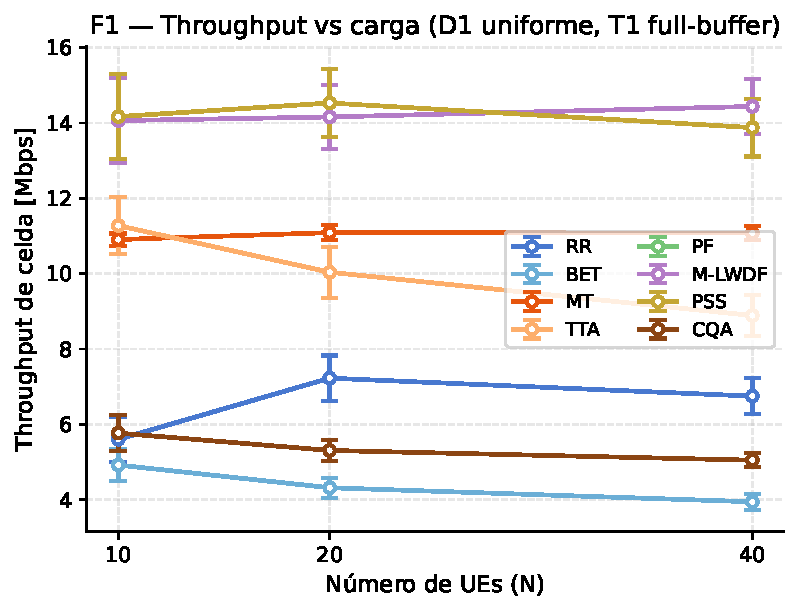
\includegraphics[width=\columnwidth]{F1_throughput_vs_N_D1.pdf}
  \caption{Throughput de celda vs N (D1, T1). PSS y PF escalan bien; BET penaliza por equidad.}
  \label{fig:f1}
\end{figure}

\begin{figure}[t]
  \centering
  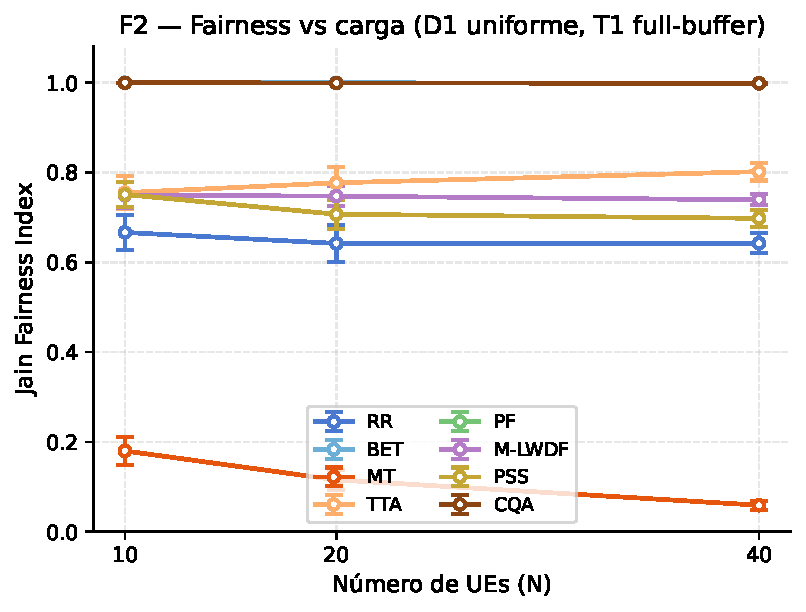
\includegraphics[width=\columnwidth]{F2_jain_vs_N_D1.pdf}
  \caption{Jain vs N (D1, T1). MT colapsa con N; TTA y PF son estables.}
  \label{fig:f2}
\end{figure}

\begin{figure}[t]
  \centering
  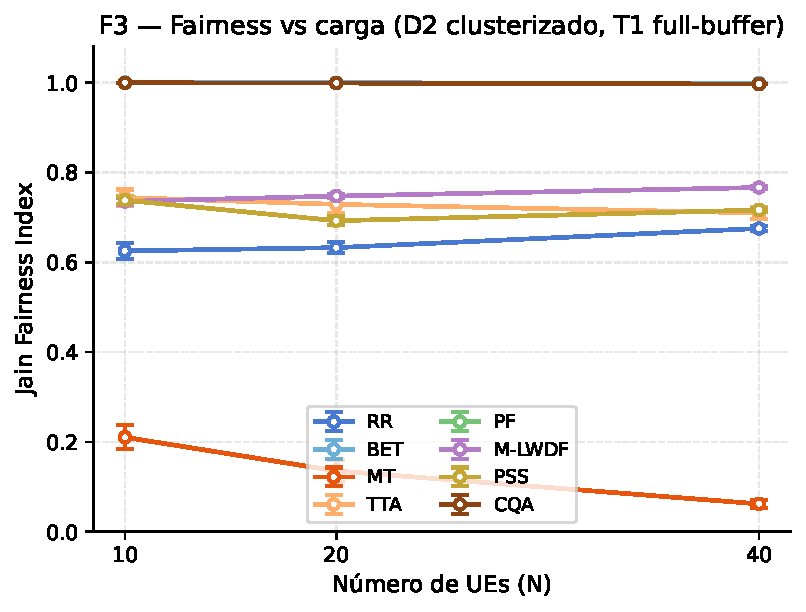
\includegraphics[width=\columnwidth]{F3_jain_vs_N_D2.pdf}
  \caption{Jain vs N (D2, T1). TTA es el único que cambia de pendiente respecto a D1.}
  \label{fig:f3}
\end{figure}

\begin{figure}[t]
  \centering
  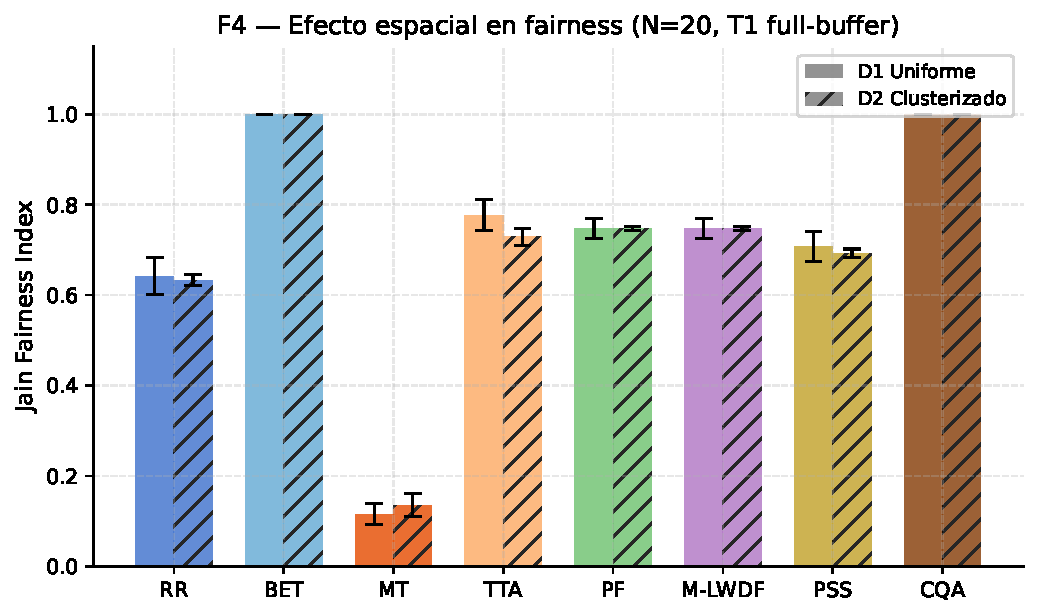
\includegraphics[width=\columnwidth]{F4_jain_D1vsD2_N20_T1.pdf}
  \caption{Jain D1 vs D2, N=20, T1. MT tiene fairness mala en ambas condiciones.}
  \label{fig:f4}
\end{figure}

H1 se confirma parcialmente: la starvation bajo D2 existe y es sistemática para MT
(los UEs de C3 a 400~m reciben cero recursos de forma consistente), pero el índice
de Jain global no lo captura bien porque MT ya era injusto en D1. La degradación
más clara de H1 aparece en TTA, no en MT.

\subsection{H2: Efecto espacial vs número de usuarios}

Esta hipótesis nos salió mal. Anticipábamos que pasar de distribución uniforme a
clusterizada (D1$\to$D2) impactaría más en la equidad que triplicar el número de
usuarios (N=10$\to$40). La Tabla~\ref{tab:h2} muestra lo contrario para 6 de 7
schedulers.

\begin{table}[t]
  \centering
  \caption{¿Qué impacta más la equidad: la distribución o la carga?}
  \label{tab:h2}
  \footnotesize
  \begin{tabular}{@{}lccc@{}}
    \toprule
    \textbf{Scheduler} & $|\Delta J|$ \textbf{espacial} & $|\Delta J|$ \textbf{carga} & \textbf{Domina} \\
    \midrule
    RR     & 0.009 & 0.024 & Carga \\
    BET    & 0.000 & 0.001 & Carga \\
    MT     & 0.020 & 0.121 & Carga \\
    TTA    & 0.048 & 0.047 & \textbf{Espacial} \\
    PF     & 0.000 & 0.011 & Carga \\
    M-LWDF & 0.000 & 0.011 & Carga \\
    PSS    & 0.015 & 0.053 & Carga \\
    \bottomrule
  \end{tabular}
\end{table}

La explicación más plausible: PF, M-LWDF y TTA normalizan el CQI instantáneo por un
historial promedio. Un UE en C3 (400~m, SINR bajo) tiene un historial bajo, pero su
ratio instantáneo/histórico puede ser tan competitivo como el de uno en C1 cuando el
fading lo favorece. El historial actúa como igualador automático de ventajas de canal.
Agregar más usuarios, en cambio, satura progresivamente la celda y hace más difícil
servir a todos ---ahí sí hay un deterioro consistente.

Para MT la diferencia es aplastante: $\Delta J_{carga}=0.121$ vs $\Delta J_{espacial}=0.020$.
Triplicar los usuarios es seis veces más dañino para la equidad de MT que pasar a
clusters. Con N=40 hay 40 candidatos para el mejor canal en cada TTI: las chances de
que un mismo usuario gane dos TTIs consecutivos son mínimas, pero la probabilidad de
que los del cluster C3 nunca ganen sube.

El único scheduler donde el efecto espacial marginalemente domina es TTA, por las
razones descritas en H1. Es el único cuya métrica de normalización (tasa wideband del
mismo TTI) no acumula historial y por tanto no compensa la desventaja geográfica tan
eficientemente.

Este resultado tiene una implicación práctica concreta: si un operador quiere mejorar
la equidad en una celda, debe preocuparse primero por la carga (¿está saturada?) antes
que por la geometría de los usuarios. PF absorbe la heterogeneidad espacial sin
configuración adicional.

\subsection{H3: Efecto del tráfico heterogéneo}

Aquí aparece el resultado más contraintuitivo del trabajo. Al introducir tráfico
heterogéneo (T2), el throughput de celda cae en todos los schedulers (Fig.~\ref{fig:f5}).
Lo esperable. Lo inesperado es \emph{quién cae más}: M-LWDF baja un 31.2\% y PSS un
26.9\%, mientras que MT ---el más agresivo en maximizar throughput--- casi no se mueve
(-1.2\%).

\begin{figure}[t]
  \centering
  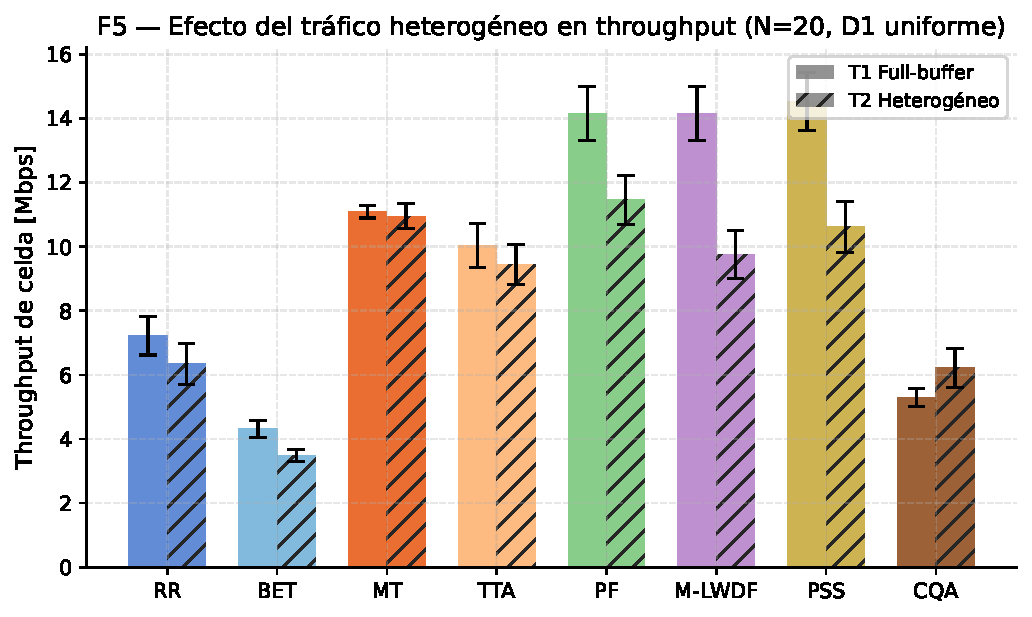
\includegraphics[width=\columnwidth]{F5_throughput_T1vsT2_N20_D1.pdf}
  \caption{Throughput total: T1 vs T2 (N=20, D1). La paradoja: M-LWDF cae más que cualquier otro.}
  \label{fig:f5}
\end{figure}

La razón es estructural. M-LWDF prioriza flujos según su delay head-of-line ponderado
por la PLR objetivo. Los flujos GBR de video (1.5~Mbps) y gaming (64~kbps) tienen
restricciones de delay muy estrictas, así que M-LWDF les asigna recursos
agresivamente aunque tengan tasas bajas. El resultado: los flujos best-effort quedan
relegados, y el throughput \emph{total} de la celda cae porque se dedica capacidad a
flujos de baja tasa que no la usan toda. M-LWDF hace exactamente lo que fue diseñado
para hacer; el "costo" es que el throughput agregado baja.

MT, en contraste, ignora completamente el tipo de bearer. Para él, un paquete de video
y uno de BE son indistinguibles: solo importa el CQI instantáneo. Por eso su throughput
apenas cambia entre T1 y T2. Claro que tampoco cumple los SLA de los flujos GBR, pero
eso no aparece en el throughput total.

La Fig.~\ref{fig:f6} lo hace explícito: M-LWDF y PSS transfieren capacidad desde BE
hacia GBR. PF distribuye ambos proporcionalmente sin distinguirlos.

\begin{figure}[t]
  \centering
  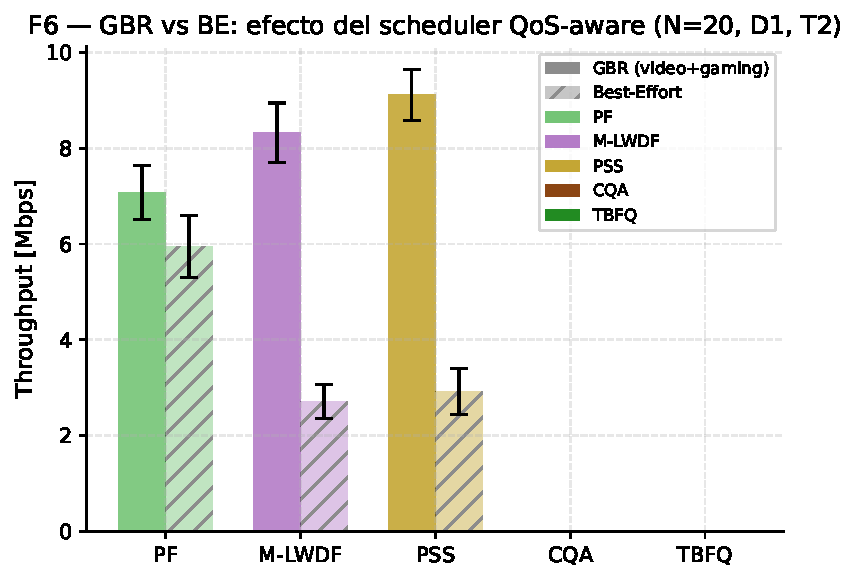
\includegraphics[width=\columnwidth]{F6_GBR_vs_BE_N20_D1_T2.pdf}
  \caption{Throughput GBR vs BE bajo T2. M-LWDF favorece GBR; PF no distingue entre tipos.}
  \label{fig:f6}
\end{figure}

La diferencia entre T1 y T2 para PF es estadísticamente significativa
($t=+4.96$, $p<0.001$, $d=1.57$), y H3 se confirma. Pero el matiz importante
es que la caída no viene de que PF sea ineficiente: viene de que el tráfico GBR
tiene tasas máximas garantizadas más bajas que el best-effort full-buffer.

\subsection{H4: Schedulers QoS-aware bajo tráfico heterogéneo}

La Fig.~\ref{fig:f8} es la más interesante del paper. Muestra el índice de Jain bajo
T2 ---tráfico heterogéneo--- para D1 y D2. Cuando los usuarios están distribuidos
uniformemente (D1), los tres schedulers QoS-aware tienen Jain similar: PF 0.561,
M-LWDF 0.564, PSS 0.553. La diferencia es mínima y no significativa.

Cuando los usuarios están clusterizados (D2), las líneas se separan. PF baja a 0.543.
M-LWDF y PSS suben a 0.596. La brecha es estadísticamente sólida ($p<0.001$, $d\approx5$;
Tabla~\ref{tab:h4}).

\begin{figure}[t]
  \centering
  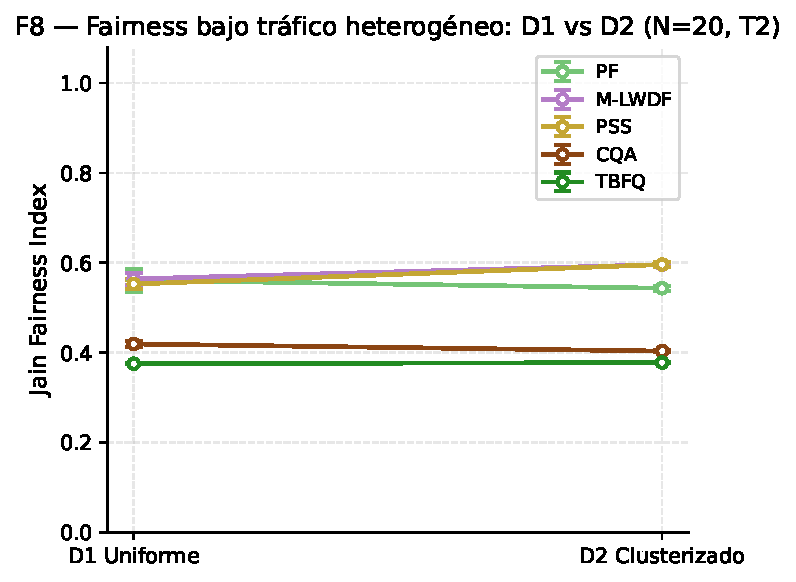
\includegraphics[width=\columnwidth]{F8_jain_D1vsD2_N20_T2.pdf}
  \caption{Jain bajo T2: M-LWDF y PSS \emph{mejoran} con D2; PF empeora. Las líneas se cruzan.}
  \label{fig:f8}
\end{figure}

\begin{table}[t]
  \centering
  \caption{Welch $t$-test: Jain T2, N=20, D2. El efecto M-LWDF/PSS vs PF es grande.}
  \label{tab:h4}
  \footnotesize
  \begin{tabular}{@{}lcccc@{}}
    \toprule
    \textbf{Comparación} & $\bar{A}$ & $\bar{B}$ & $p$ & $d$ \\
    \midrule
    M-LWDF vs PF & 0.596 & 0.543 & $<$0.001 & +5.14 \\
    PSS vs PF    & 0.596 & 0.543 & $<$0.001 & +4.72 \\
    PSS vs M-LWDF & 0.596 & 0.596 & 0.953 & +0.02 \\
    \bottomrule
  \end{tabular}
\end{table}

Por qué M-LWDF y PSS \emph{mejoran} su Jain al pasar a D2: con distribución interleaved,
cada cluster tiene un tercio de flujos GBR. Los UEs GBR en C3 (400~m, canal débil)
acumulan delay HOL rápidamente porque PF no les da prioridad. M-LWDF escala su prioridad
precisamente cuando ese delay crece, así que los UEs de C3 eventualmente reciben
recursos aunque su canal sea malo. Al servir a más UEs distantes, el Jain global sube.
PF no tiene ese mecanismo: como el canal de C3 siempre pierde contra C1 en la métrica
proporcional, sus UEs quedan rezagados.

El retardo E2E (Fig.~\ref{fig:f7}) no diferencia entre schedulers de forma significativa
(todos en torno a 3.2--3.3~ms, muy por debajo de los 50~ms de SLA para gaming y los
300~ms para video). Bajo la carga evaluada, el cuello de botella está en el canal, no
en el buffer del scheduler.

\begin{figure}[t]
  \centering
  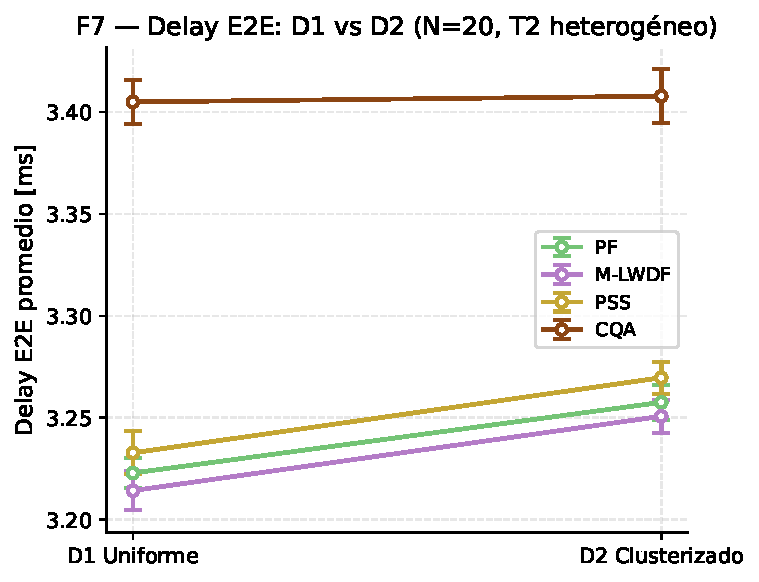
\includegraphics[width=\columnwidth]{F7_delay_D1vsD2_N20_T2.pdf}
  \caption{Retardo E2E: D1 vs D2 (N=20, T2). Ningún scheduler viola los SLA de latencia.}
  \label{fig:f7}
\end{figure}

% =============================================================================
\section{Discusión}
\label{sec:discusion}

El resultado más claro de este trabajo no es cuál scheduler es mejor ---eso depende
del escenario--- sino cuáles supuestos del diseño del scheduler determinan su
comportamiento bajo heterogeneidad.

PF es robusto porque normaliza por historial propio: si un UE lleva varios TTIs sin
recursos, su ratio instantáneo/histórico sube y eventualmente le toca. Es una forma
de equidad que no requiere conocer el tipo de tráfico ni configurar umbrales.
El precio es que no distingue entre un paquete de video con restricción de latencia
y uno de descarga en segundo plano.

M-LWDF añade exactamente esa distinción: el delay HOL pondera la prioridad según
urgencia. Pero hacerlo tiene un costo en throughput total cuando el tráfico GBR
tiene tasas garantizadas bajas ---el scheduler dedica recursos a flujos que no los
usan completamente, y el best-effort no puede aprovechar ese margen.

Lo que más nos sorprendió al analizar los resultados es el comportamiento de BET
bajo saturación. Jain=0.999 en todas las condiciones, incluyendo D2 con clusters.
BET logra equidad perfecta siendo ignorante del canal: simplemente acumula throughput
histórico por UE y da tiempo a quien menos ha recibido. Es el algoritmo más simple
de la taxonomía y el más equitativo. El costo ---4.3~Mbps de throughput de celda
frente a los 14.5~Mbps de PSS--- es enorme, pero si el caso de uso requiere
equidad por encima de eficiencia (por ejemplo, IoT con muchos dispositivos de
baja tasa), BET lo resuelve sin configuración.

MT es el único que no debería usarse en una celda heterogénea con múltiples servicios.
En D2 con tráfico interleaved, los UEs de C3 reciben cero bytes de forma sistemática.
No es un problema del fading; es por diseño: MT nunca considerará a un UE lejano si
hay uno cercano con mejor canal. En los experimentos, 14 de 20 UEs quedaron sin
servicio durante toda la simulación.

\textbf{Sobre las limitaciones.} Este experimento usa una sola celda y usuarios estáticos.
La interferencia inter-celda puede cambiar el ranking de schedulers: M-LWDF, que aquí
compite solo por recursos internos, en entornos multi-celda enfrenta además interferencia
de celdas vecinas, lo que amplifica el delay HOL y potencialmente exagera su ventaja
---o la revierte si la interferencia domina sobre el canal. Esto queda como pregunta
abierta para trabajo futuro.

% =============================================================================
\section{Conclusiones}
\label{sec:conclusiones}

La pregunta central de este trabajo era si existe algún scheduler capaz de satisfacer
simultáneamente throughput, equidad y QoS en una celda heterogénea. La respuesta
directa es no. Ninguno de los siete algoritmos evaluados domina en todas las métricas
bajo todas las condiciones. Lo que sí existe son schedulers mejores para contextos
específicos.

Si el tráfico es homogéneo y la prioridad es eficiencia con equidad razonable, PF
sigue siendo la elección correcta. No requiere configuración de parámetros de QoS,
es robusto a la distribución espacial de los usuarios, y su rendimiento es prácticamente
indistinguible de M-LWDF cuando no hay restricciones de latencia diferenciadas.

Si el tráfico mezcla flujos GBR con best-effort, y especialmente si los usuarios están
agrupados en zonas de distinta calidad de canal, M-LWDF y PSS ofrecen una ventaja
real en equidad global. La ganancia no es gratuita: ambos reducen el throughput total
de la celda entre un 27 y un 31\% porque priorizan flujos de baja tasa. Esa es la
decisión que el operador tiene que tomar: ¿prefiero maximizar el throughput agregado
o garantizar que los usuarios con peor canal reciban servicio?

El resultado más valioso ---porque no lo anticipamos--- es que la carga de la celda
afecta más la equidad que la distribución geográfica de los usuarios, al menos cuando
se usan schedulers channel-aware. Eso significa que antes de preocuparse por si los
usuarios están clusterizados o dispersos, un operador debería revisar si la celda está
saturada. Un PF en una celda al 90\% de carga es más injusto que en una al 50\%,
independientemente de dónde estén físicamente los usuarios.

Quedan preguntas sin responder. La principal: ¿cómo cambia este panorama con
interferencia inter-celda? La celda única de este experimento aisló los efectos del
scheduler puro, pero en redes densas la interferencia puede hacer que un UE en el
borde de la celda tenga SINR negativo sin importar qué scheduler use. En ese escenario,
M-LWDF podría amplificar su ventaja ---o ser insuficiente. Esa extensión justifica
un experimento por sí sola.

% =============================================================================
\section*{Agradecimientos}

Los experimentos descritos en este trabajo requirieron aproximadamente 30 horas de
cómputo distribuido. El autor agradece al grupo de Redes de Computadoras de la BUAP
por el acceso a la infraestructura utilizada.

% =============================================================================
\bibliographystyle{IEEEtran}
\bibliography{references}

\end{document}
